\chapter{Extending AdaptaBERT with Next Sentence Prediction} \label{chap:extending-adaptabert}

In Chapter \ref{chap:domain-adaptation} we described the AdaptaBERT model, and measured its performance for the political bias detection task on our cross-domain Reddit dataset. We now extend AdaptaBERT by adding a Next Sentence Prediction stage to its fine-tuning stages, and assess the performance of the new model on political bias detection and named entity recognition tasks.

\section{Motivation}

Currently, AdaptaBERT only adds an extra masked language modelling objective to the training stages of BERT. However, standard BERT undergoes two pretraining objectives to train its contextualised word embeddings - masked language modelling (MLM) and next sentence prediction (NSP). The original BERT paper \cite{bert} states that the MLM objective is used to train a deep bidirectional internal representation of the words, and NSP is used mainly to help improve BERT's performance on question answering (QA) and natural language inference (NLI) tasks.

Intuitively this makes sense - tuning BERT's internal representations to better understand context between sentences will help it perform better at tasks which require scanning long sequences of text, such as QA and NLI. However, our cross-domain dataset of articles and Reddit comments also contains samples with long text sequences - each article in our dataset contains 31 sentences on average. Comments are less sentence-heavy, with each comment containing on average 2 sentences. Both domains show heavy right-hand skew in the distribution of number of sentences (see Figure \ref{fig:num-sentences-distributions}).

\begin{figure}[ht]
    \centering
    \begin{subfigure}{\textwidth}
        \centering
        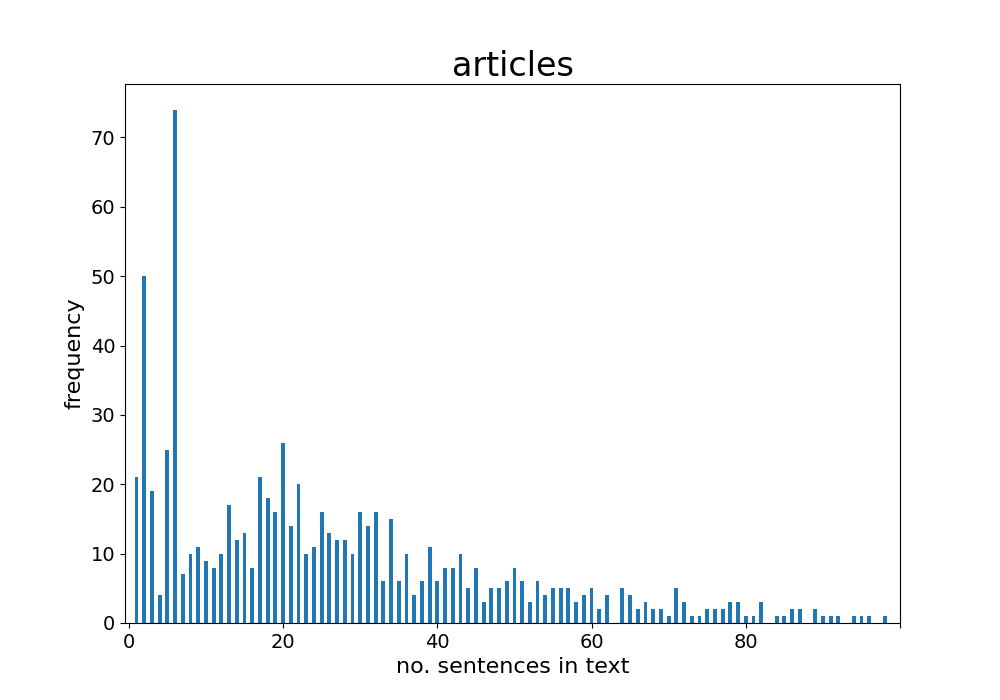
\includegraphics[scale=0.45]{0-img/num-sentences-distribution-articles.png}
    \end{subfigure}
    \begin{subfigure}{\textwidth}
        \centering
        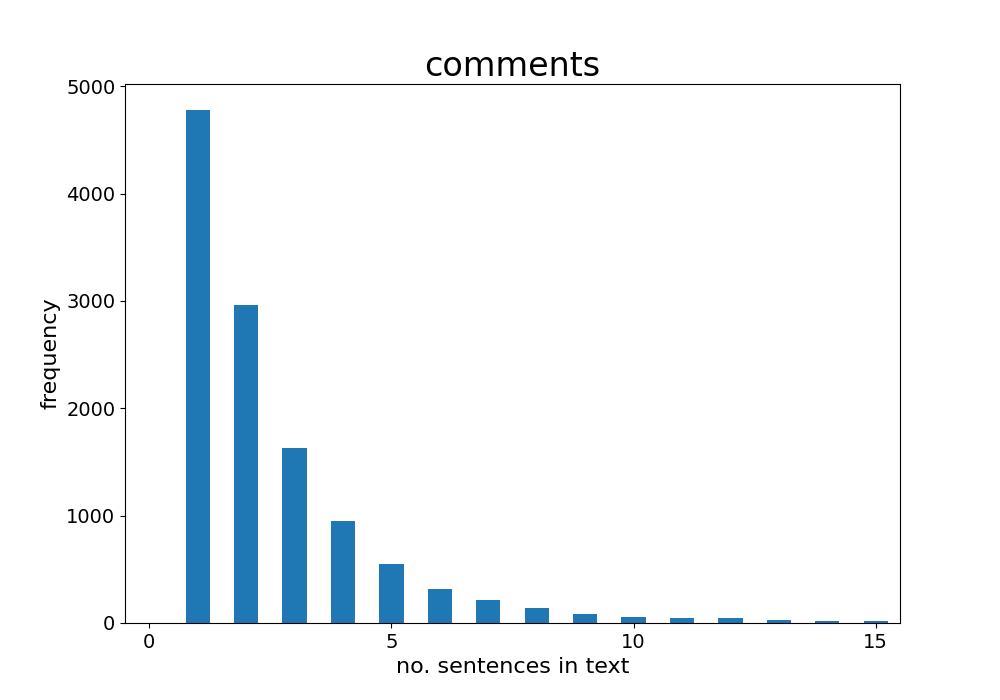
\includegraphics[scale=0.45]{0-img/num-sentences-distribution-comments.png}
    \end{subfigure}
    \caption{Distribution of number of sentences in each article (top) and comment (bottom) in our Reddit dataset}
    \label{fig:num-sentences-distributions}
\end{figure}

We explore extending AdaptaBERT by adding a Next Sentence Prediction stage directly after the MLM stage, to see if this improves classification performance. Our hypothesis is that this will improve performance in the \textit{comments $ \rightarrow $ articles} scenario, since in this case the target domain contains textual content with many sentences per sample (31 on average), however the performance benefit will not be so great for \textit{articles $ \rightarrow $ comments}, since the target domain in this case doesn't exhibit many sentences per sample. The architecture we propose is shown in Figure \ref{fig:adaptabert-nsp}, compared against standard AdaptaBERT and previous approaches.

\begin{figure}
    \centering
    \hspace{-1.5cm}
    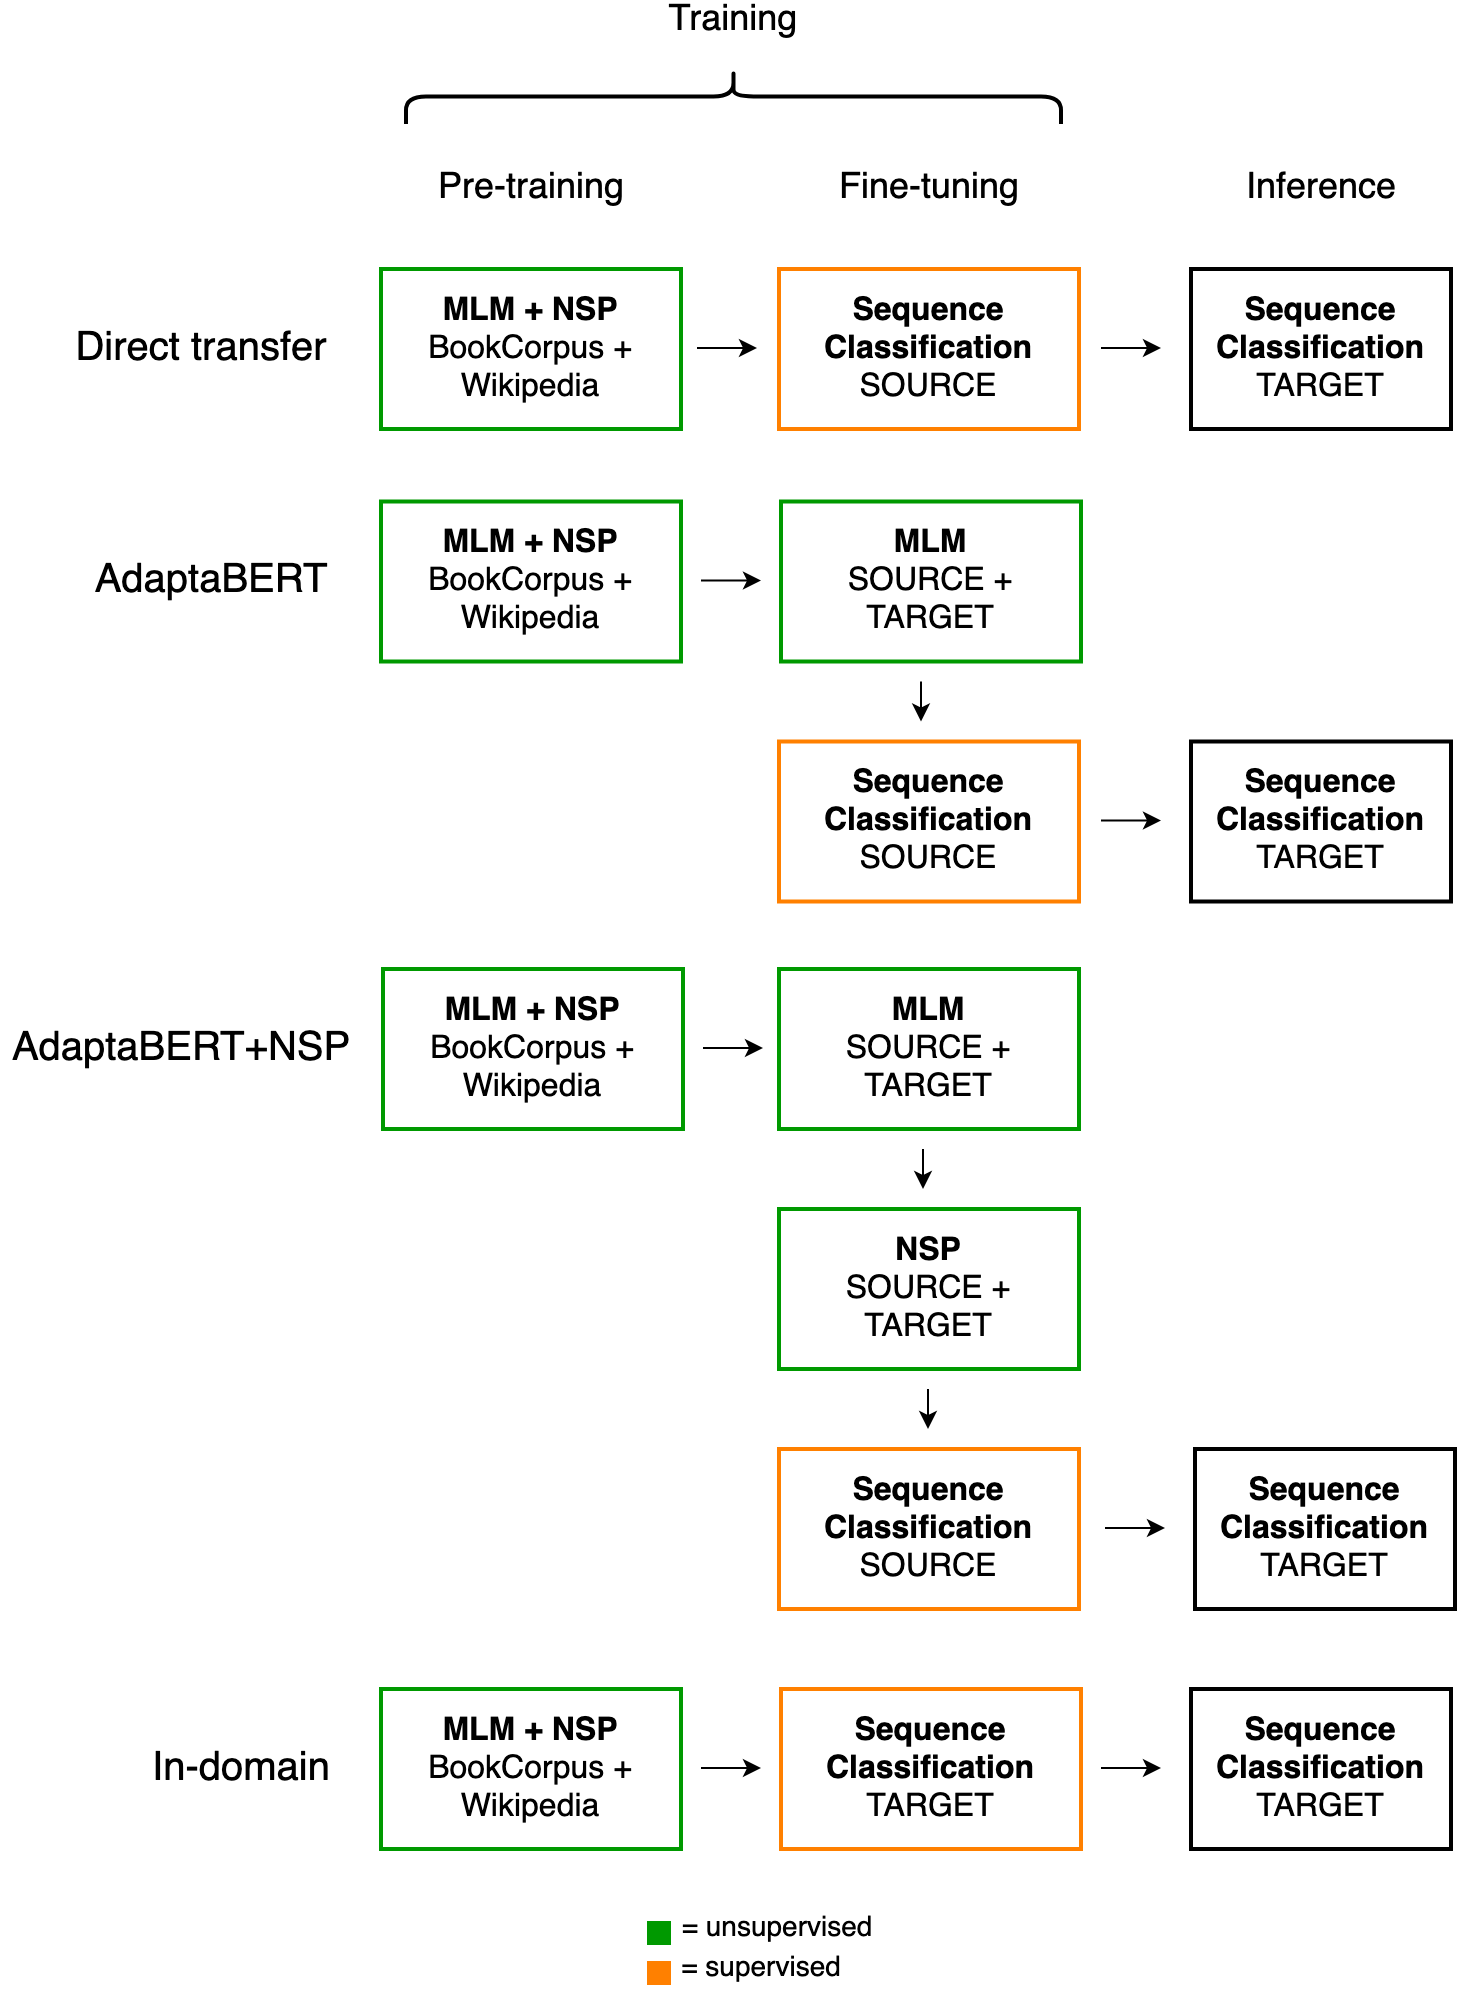
\includegraphics[scale=0.28]{0-img/adaptabert-nsp.png}
    \caption{AdaptaBERT extended with the NSP stage, compared to standard AdaptaBERT, direct transfer and in-domain approaches}
    \label{fig:adaptabert-nsp}
\end{figure}

\section{Implementing next sentence prediction}

In the original BERT paper \cite{bert}, NSP is implemented by creating sentence pair examples \texttt{<A, B>} out of the pre-training corpus where 50\% of the time sentence B is actually the sentence that follows A in the corpus, and the other 50\% of the time it is a randomly-selected sentence. BERT is then trained for a binary classification objective to determine for each sentence pair whether sentence B actually follows sentence A or not. We mirror this methodology for our extended AdaptaBERT.

Similarly to standard AdaptaBERT, we use an equal amount of source domain and target domain examples in the NSP stage, up to a maximum of the entire target domain. For each article and comment in our dataset, we choose 2 sentence pairs where the second sentence actually follows the first sentence, and 2 pairs where the second sentence is instead a random sentence from the same text. This gives us a collection of NSP training examples 4x larger than the size of the target domain.

\section{Experimental setup}

We compare the performance of extended AdaptaBERT to standard AdaptaBERT in two scenarios - political bias detection with the Reddit dataset as we have been doing previously, and also the named entity recognition (NER) task explored by Han \& Eisenstein in the original AdaptaBERT paper \cite{adaptabert}.

The NER task is an example of a token classification task - so far, we have only explored sequence classification for political bias detection. Han \& Eisenstein explore transfer from news content to tweets, using the CoNLL-2003 and WNUT 2016 NER datasets. The CoNLL dataset \cite{conll} is a corpus of 1,393 Reuters news stories \cite{reuters} taken between August 1996 and August 1997, and the WNUT NER dataset \cite{wnut} (taken from the Workshop of Noisy User Text 2016) is a collection of 3,819 generic tweets sampled from between December 2014 and February 2015. Both datasets are annotated at the token level by named entity (e.g. company, person, TV show, etc).

When tuning hyperparameters, we achieve best performance on both tasks when using only 1 epoch for the NSP stage. We use 5 epochs for MLM and sequence classification fine-tuning, as in Section \ref{sec:adaptabert}. We also use a source proportion of $ \frac{1}{3} $ for the MLM stage, as we found in Section \ref{subsec:src-proportion-adaptabert} that this gives the best performance for standard AdaptaBERT.

\section{Evaluation for political bias detection task} \label{sec:nsp-evaluation-political-bias}

As in Chapter \ref{chap:domain-adaptation}, we report results for both \textit{articles $ \rightarrow $ comments} transfer and \textit{comments $ \rightarrow $ articles} transfer. Results are shown in Table \ref{tab:adaptabert-nsp-results}.

\begin{table}[ht]
    \begin{center}
        \begin{tabular}{|c|c|c|c|c|c|}
            \hline
            \multicolumn{3}{|c|}{\textbf{Task}} & \multicolumn{3}{|c|}{Bias detection} \\
            \hline
            \multicolumn{3}{|c|}{\textbf{Transfer direction}} & \multicolumn{3}{|c|}{Articles $ \rightarrow $ comments} \\
            \hline \hline
            \multicolumn{2}{|c|}{\textbf{Model Type}} & \multicolumn{2}{|c|}{\textbf{Macro-F1}} & \multicolumn{2}{|c|}{\textbf{Accuracy}} \\
            \hline
            \multicolumn{2}{|c|}{Direct transfer} & \multicolumn{2}{|c|}{54.4} & \multicolumn{2}{|c|}{51.8} \\
            \multicolumn{2}{|c|}{AdaptaBERT} & \multicolumn{2}{|c|}{58.0} & \multicolumn{2}{|c|}{59.2} \\
            \multicolumn{2}{|c|}{AdaptaBERT+NSP} & \multicolumn{2}{|c|}{58.0} & \multicolumn{2}{|c|}{58.1} \\
            \hline
            \multicolumn{2}{|c|}{In-domain} & \multicolumn{2}{|c|}{67.2} & \multicolumn{2}{|c|}{67.6} \\
            \hline
        \end{tabular}
    \end{center} \vspace{10pt}
    \begin{center}
        \begin{tabular}{|c|c|c|c|c|c|}
            \hline
            \multicolumn{3}{|c|}{\textbf{Task}} & \multicolumn{3}{|c|}{Bias detection} \\
            \hline
            \multicolumn{3}{|c|}{\textbf{Transfer direction}} & \multicolumn{3}{|c|}{Comments $ \rightarrow $ articles} \\
            \hline \hline
            \multicolumn{2}{|c|}{\textbf{Model Type}} & \multicolumn{2}{|c|}{\textbf{Macro-F1}} & \multicolumn{2}{|c|}{\textbf{Accuracy}} \\
            \hline
            \multicolumn{2}{|c|}{Direct transfer} & \multicolumn{2}{|c|}{69.6} & \multicolumn{2}{|c|}{69.3}  \\
            \multicolumn{2}{|c|}{AdaptaBERT} & \multicolumn{2}{|c|}{74.0} & \multicolumn{2}{|c|}{74.1} \\
            \multicolumn{2}{|c|}{AdaptaBERT+NSP} & \multicolumn{2}{|c|}{70.9} & \multicolumn{2}{|c|}{71.0} \\
            \hline
            \multicolumn{2}{|c|}{In-domain} & \multicolumn{2}{|c|}{76.2} & \multicolumn{2}{|c|}{76.5}  \\
            \hline
        \end{tabular}
    \end{center}
    \caption{Evaluation metrics comparing extended AdaptaBERT to standard AdaptaBERT, direct transfer and in-domain baselines for the political bias detection task}
    \label{tab:adaptabert-nsp-results}
\end{table}

We can see that in both transfer directions, the extended AdaptaBERT fails to improve over the standard AdaptaBERT in both F1 score and accuracy, although it is able to match F1 score in the \textit{articles $ \rightarrow $ comments} case. In the \textit{comments $ \rightarrow $ articles} case, performance almost deteriorates to the same level as direct transfer. This suggests our hypothesis that adding Next Sentence Prediction would help classifier performance is false, regardless of which domain is the target domain. Our results seem to indicate that performance deteriorates the most when the domain with most sentences per example (i.e. articles) is the target domain, however more experiments on different datasets are ideally needed to test this hypothesis.

\section{Evaluation for NER task} \label{sec:nsp-evaluation-ner}

We only evaluate \textit{articles $ \rightarrow $ tweets} transfer, since this is the only transfer direction evaluated by Han \& Eisenstein \cite{adaptabert}. They also only provide F1 score and not accuracy. Results are shown in Table \ref{tab:adaptabert-nsp-ner-results}.

\begin{table}[ht]
    \begin{center}
        \begin{tabular}{|c|c|}
            \hline
            \textbf{Task} & NER \\
            \hline
            \textbf{Transfer direction} & Articles $ \rightarrow $ tweets \\
            \hline \hline
            \textbf{Model Type} & \textbf{Macro-F1} \\
            \hline
            Direct transfer & 57.7  \\
            AdaptaBERT & 58.9  \\
            AdaptaBERT+NSP & 61.4  \\
            \hline
            In-domain & 64.3 \\
            \hline
        \end{tabular}
    \end{center}
    \caption{Evaluation metrics comparing extended AdaptaBERT to standard AdaptaBERT, direct transfer and in-domain baselines for the NER task. Results 1, 2, and 4 taken from \cite{adaptabert}.}
    \label{tab:adaptabert-nsp-ner-results}
\end{table}

We can see the extended AdaptaBERT improves over AdaptaBERT by 2.5\% in F1 score, and comes within 3\% of the in-domain baseline.

Examining the distribution of sentences in the NER dataset (see Figure \ref{fig:ner-num-sentences-distributions}), we can see in fact both domains exhibit a low number of sentences per example. The articles, rather than having been preserved as single examples, have been split up into roughly 1 sentence per example by the WNUT dataset authors. A minority of examples contain 2 or more sentences. The average number of sentences in each tweet is of course quite low, due to Twitter's 140-character tweet limit as of December 2016, the month the dataset was published.

\begin{figure}[ht]
    \centering
    \begin{subfigure}{\textwidth}
        \centering
        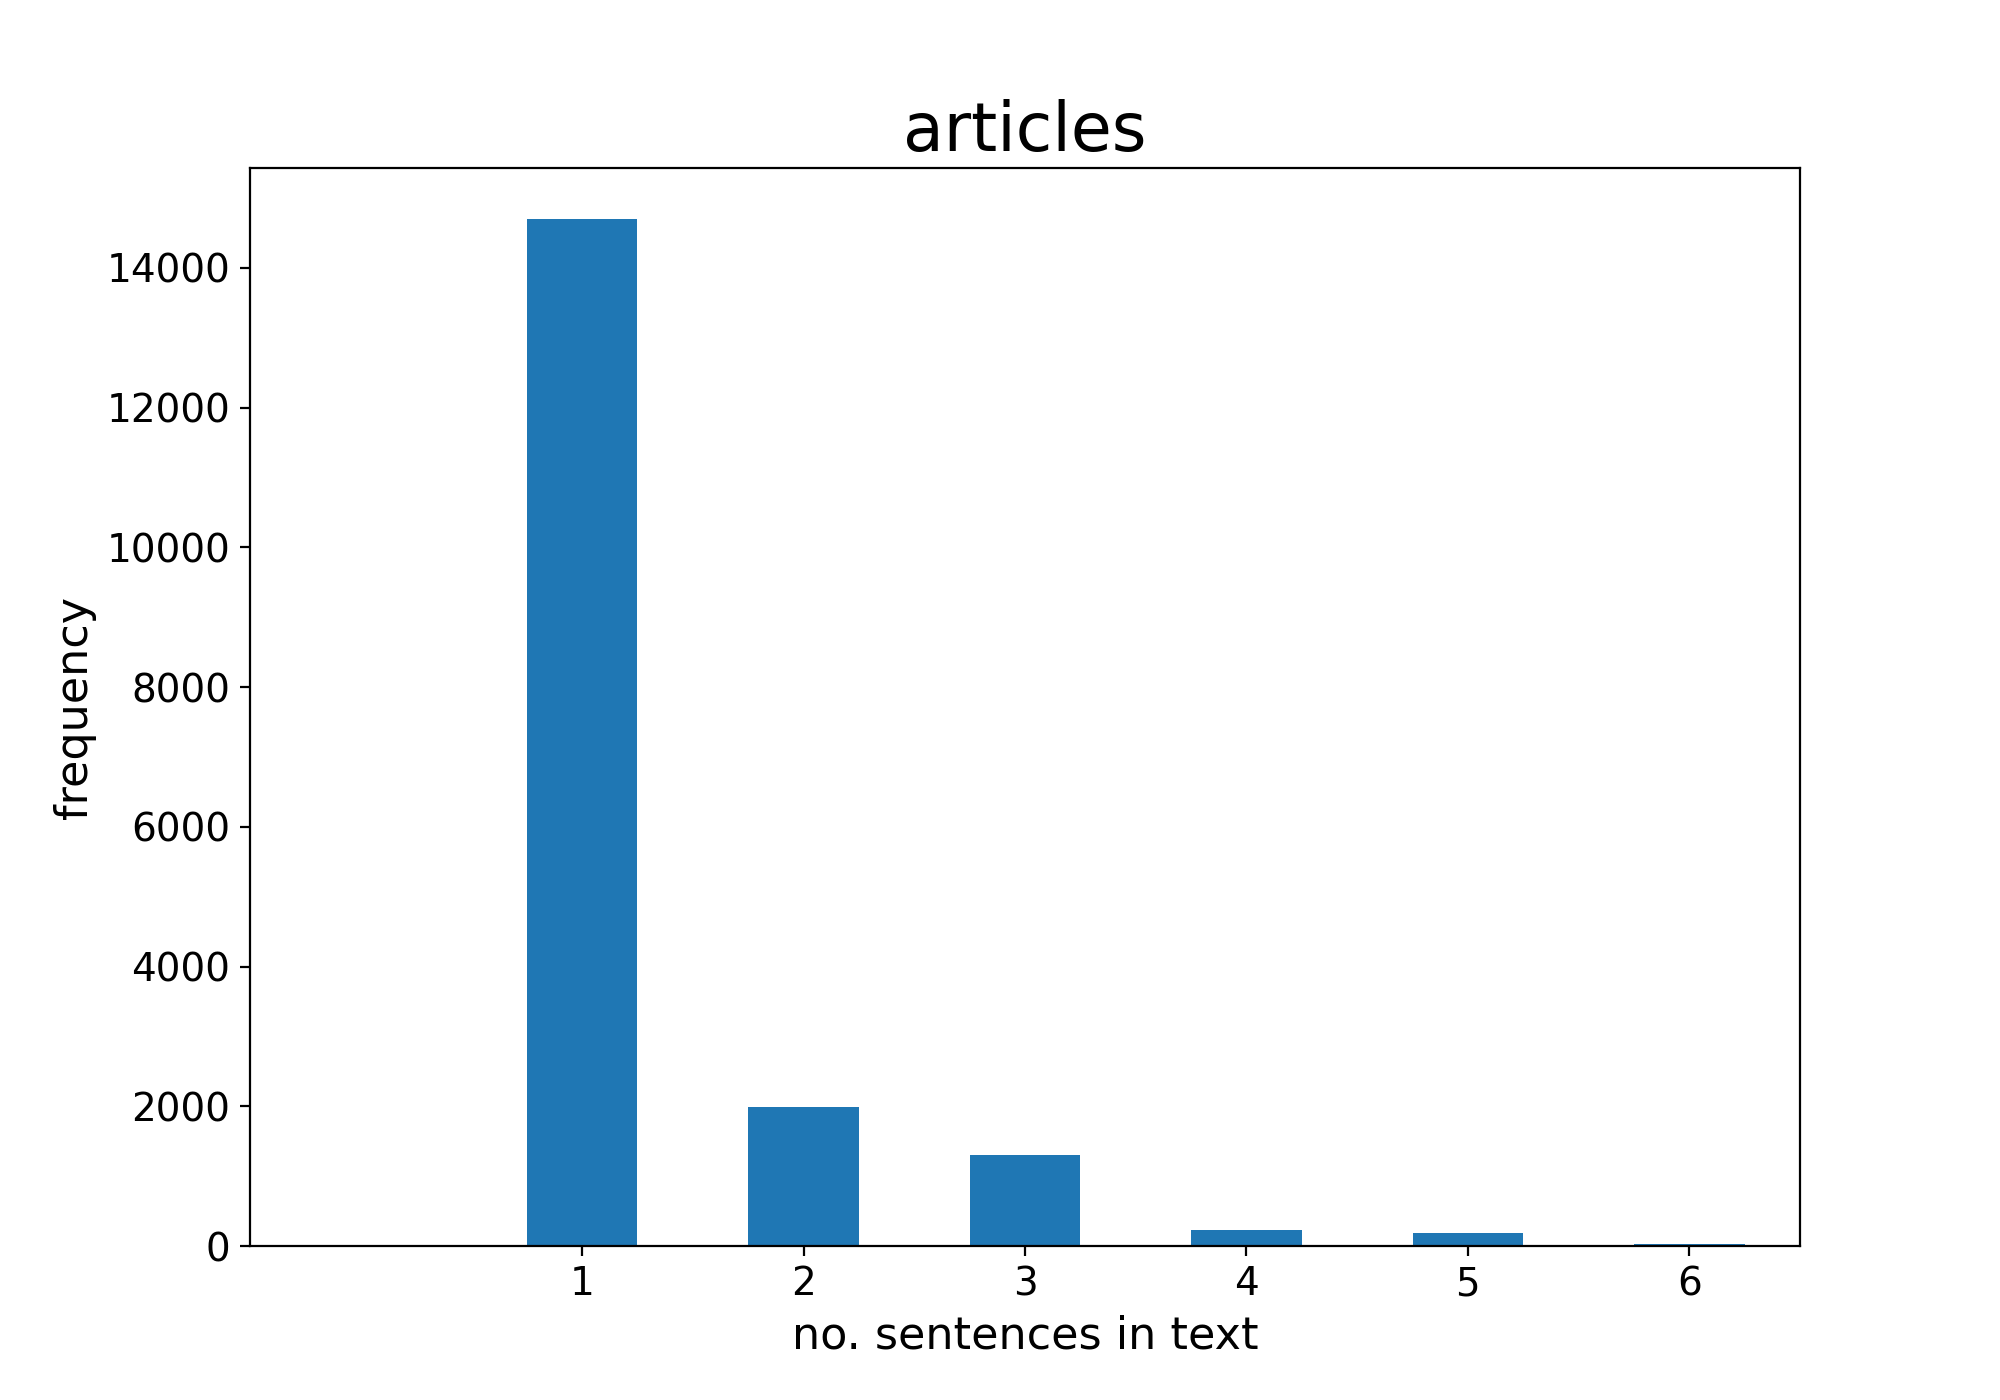
\includegraphics[scale=0.45]{0-img/ner-num-sentences-distribution-articles.png}
    \end{subfigure}
    \begin{subfigure}{\textwidth}
        \centering
        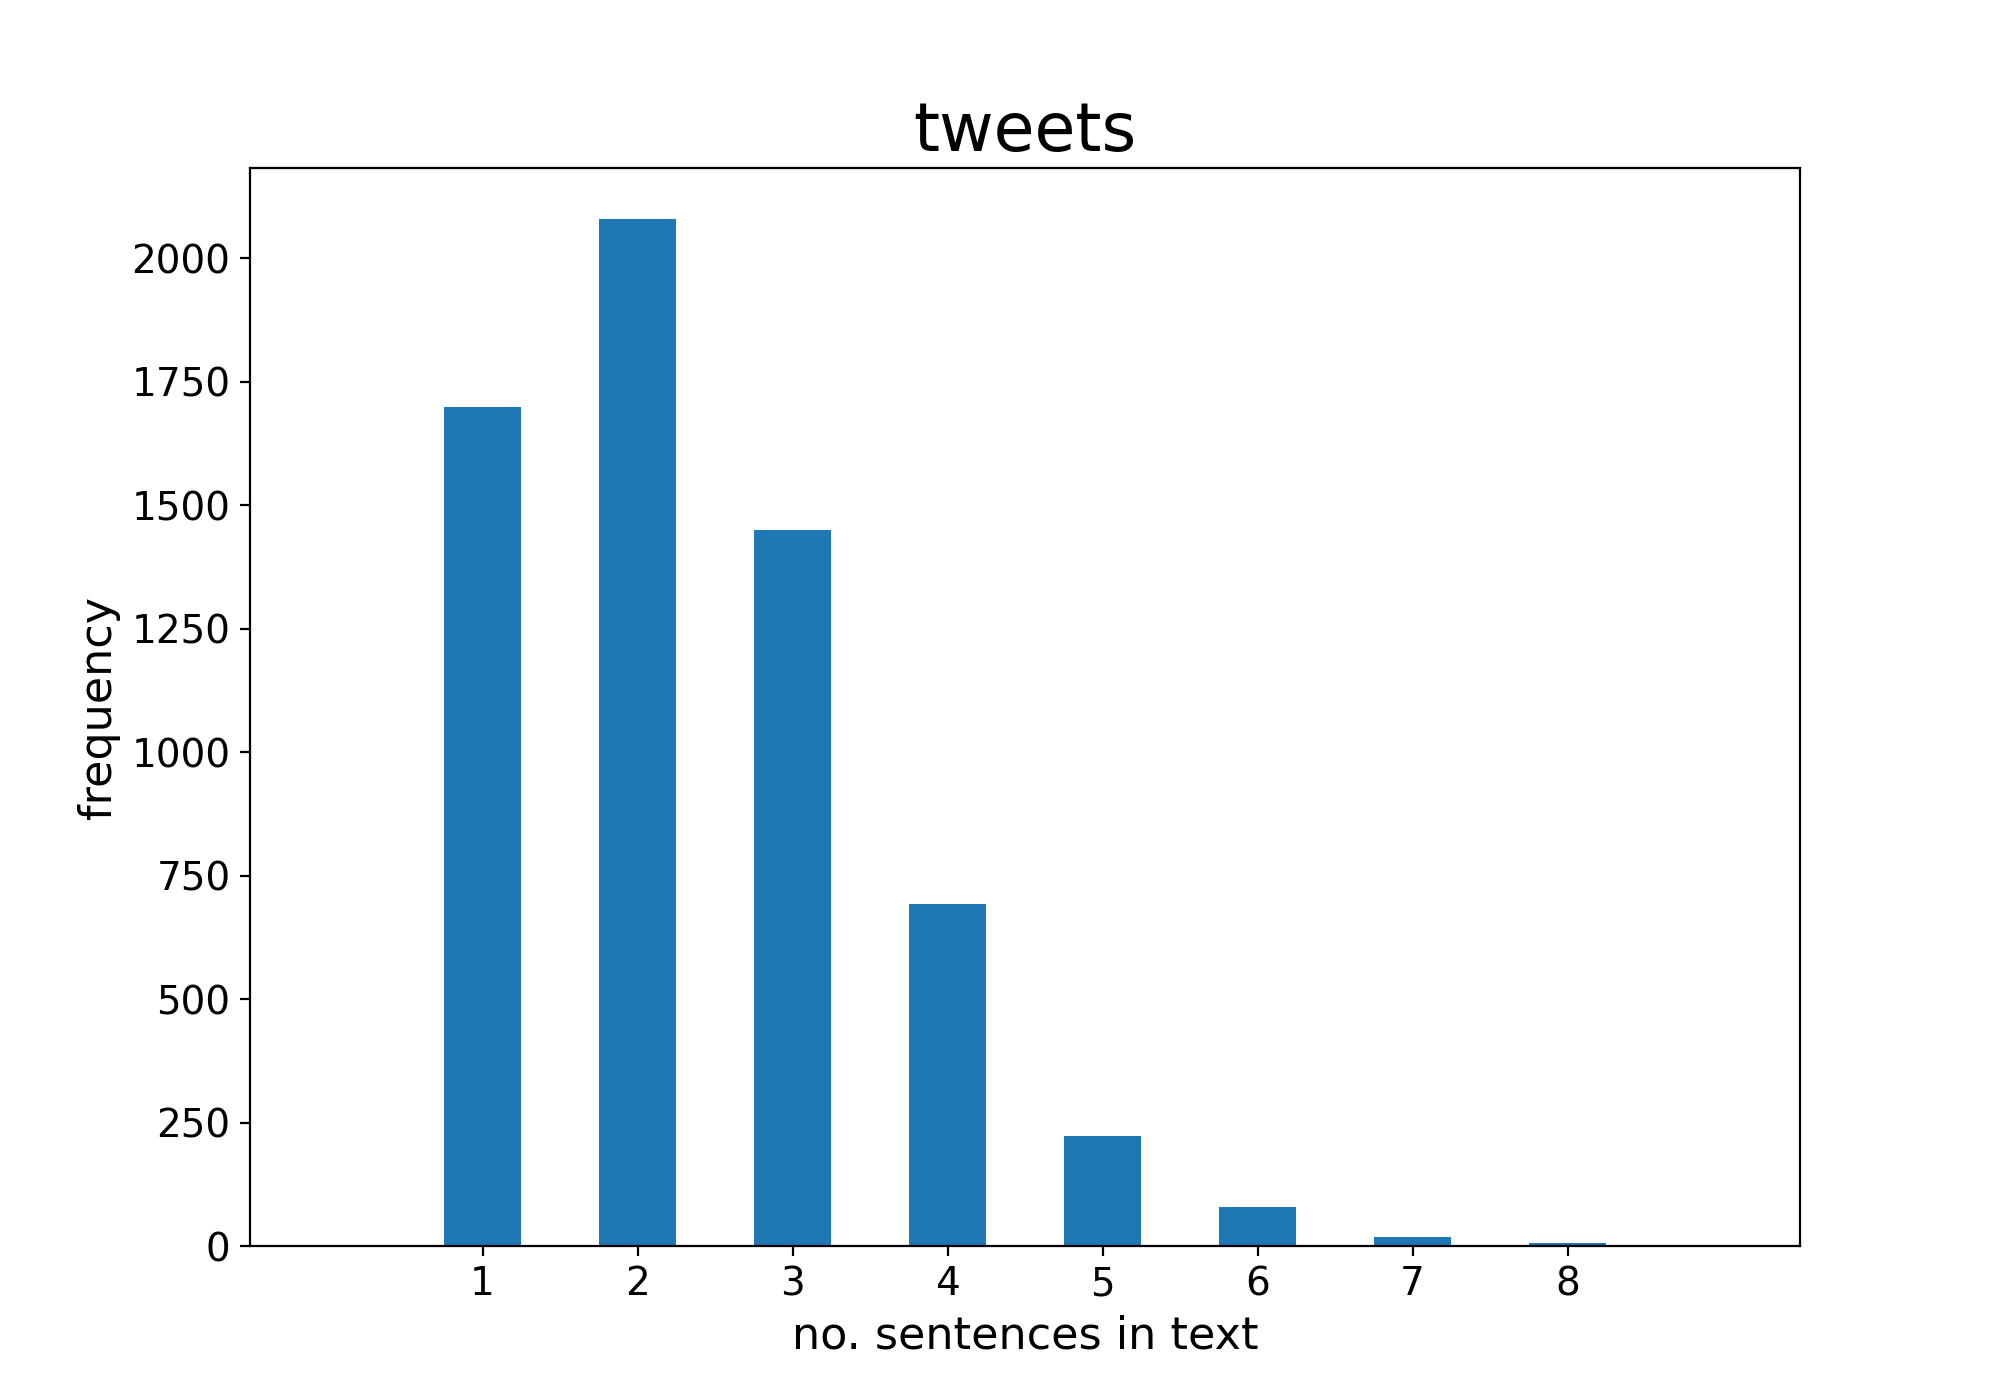
\includegraphics[scale=0.45]{0-img/ner-num-sentences-distribution-tweets.png}
    \end{subfigure}
    \caption{Distribution of number of sentences in each article (top) and tweet (bottom) in the WNUT 2016 NER dataset}
    \label{fig:ner-num-sentences-distributions}
\end{figure}

This shows us that AdaptaBERT extended with NSP can still improve over standard AdaptaBERT even when both the source and target domain exhibit a low number of sentences per training example. Based on these results and those in Section \ref{sec:nsp-evaluation-political-bias}, we hypothesis that NSP improves classifier performance when the source and target domain have \textbf{similar} distributions of number of sentences per example, irrespective of how high or low the average number of sentences per example actually is. More experimentation on different datasets is needed to fully test this hypothesis.

\section{Finding the optimal proportion of source domain examples for NSP}

In Sections \ref{sec:nsp-evaluation-political-bias} and \ref{sec:nsp-evaluation-ner}, we used an equal number of source and target domain examples for the Next Sentence Prediction stage. We now aim to find which ratio of source to target domain examples gives the optimal performance of extended AdaptaBERT, similarly to our experiments with the MLM stage in standard AdaptaBERT in Section \ref{subsec:src-proportion-adaptabert}. Again, we trial source proportion values of 0, $ \frac{1}{3} $, $ \frac{2}{3} $ and 1. In all cases we use all target domain data available.

Results for the political bias task are shown in Figure \ref{fig:nsp-src-proportion}. We can see in the \textit{articles $ \rightarrow $ comments} case we achieve the best metrics with a source proportion of 1 (i.e. using an equal amount of source and target domain data). Interestingly, in the \textit{comments $ \rightarrow $ articles} case we achieve the best metrics using no source domain material at all in the NSP stage (the F1 line is hidden behind the accuracy line between source proportions of 0 and $ \frac{1}{3} $). This gives a final F1 score of 73.5\%, compared to 70.9\% when using an equal proportion. This almost matches the performance of standard AdaptaBERT, however does not exceed it. Our results don't appear to follow the same pattern seen in Section \ref{subsec:src-proportion-adaptabert}, where adding more source domain material leads to increasing deterioration in model performance. In fact, in both transfer directions using an equal amount of source and target domain material in the NSP stage results in very good classifier performance compared to other ratios. Our new best extended AdaptaBERT results for this task are shown in Table \ref{tab:adaptabert-nsp-results-best}. 

Results for the NER task are shown in Figure \ref{fig:nsp-ner-src-proportion}. We only evaluate \textit{articles $ \rightarrow $ tweets} in this case. We can see we achieve best performance with a source proportion of $ \frac{1}{3} $, similarly to our experiments in Section \ref{subsec:src-proportion-adaptabert}. This gives a final F1 score of 62.2\%, which is a 0.8\% improvement over the result in Section \ref{sec:nsp-evaluation-ner}. Overall, this is a 3.3\% improvement over standard AdaptaBERT for this task. Our new best extended AdaptaBERT results for this task are shown in Table \ref{tab:adaptabert-nsp-ner-results-best}.

\begin{figure}[ht]
    \centering
    \begin{subfigure}{\textwidth}
        \centering
        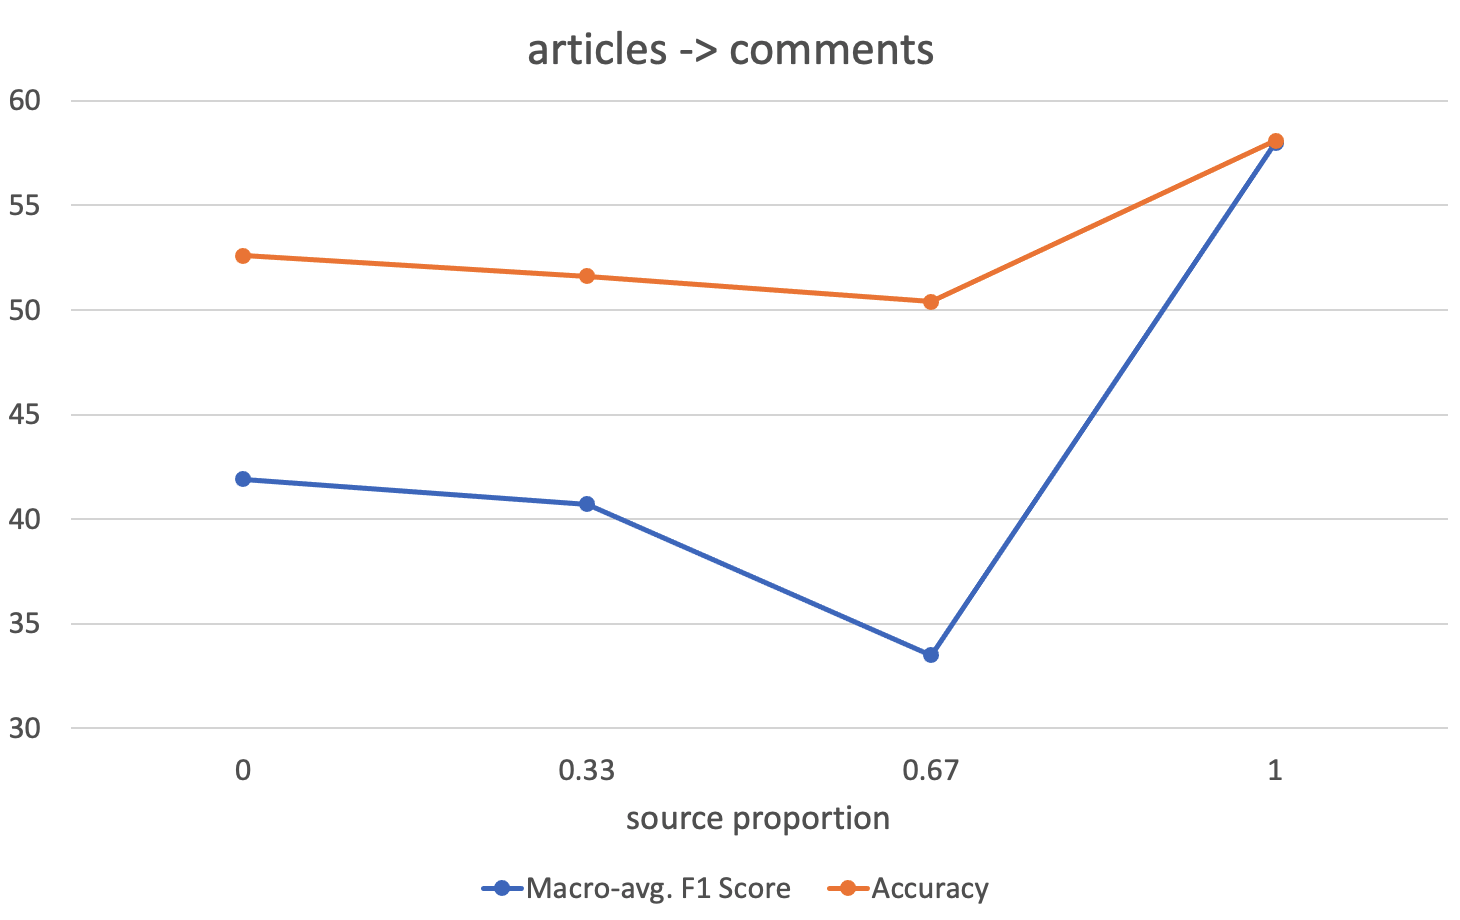
\includegraphics[scale=0.24]{0-img/nsp-src-proportion-articles-comments.png}
    \end{subfigure}
    \begin{subfigure}{\textwidth}
        \centering
        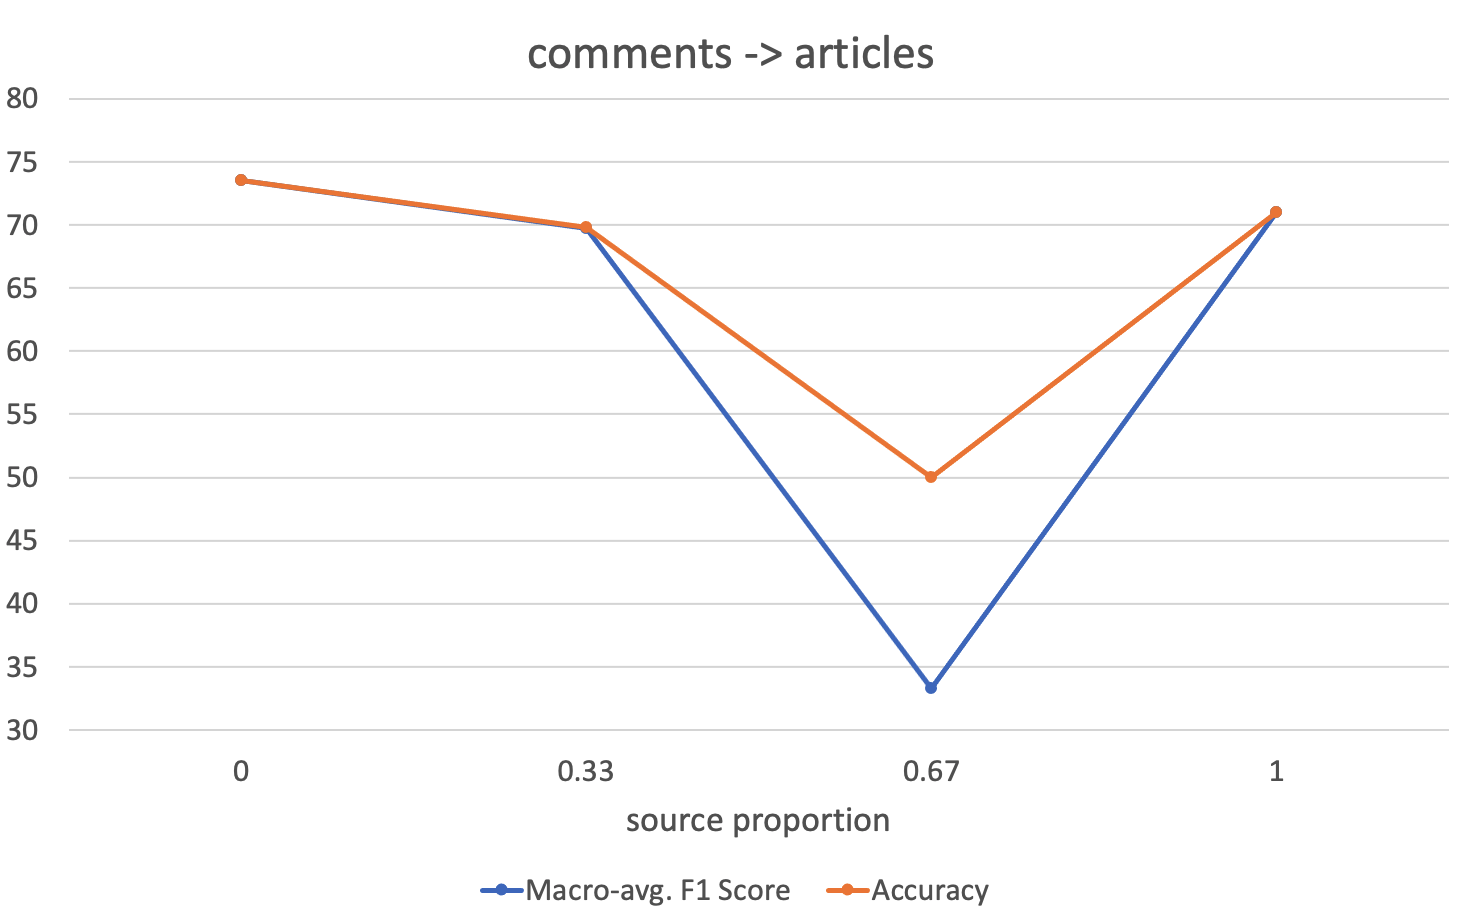
\includegraphics[scale=0.24]{0-img/nsp-src-proportion-comments-articles.png}
    \end{subfigure}
    \caption{Performance of extended AdaptaBERT on the political bias detection task when varying proportion of source domain examples compared to target domain examples used in the NSP stage}
    \label{fig:nsp-src-proportion}
\end{figure}

\begin{figure}[ht]
    \centering
    \begin{subfigure}{\textwidth}
        \centering
        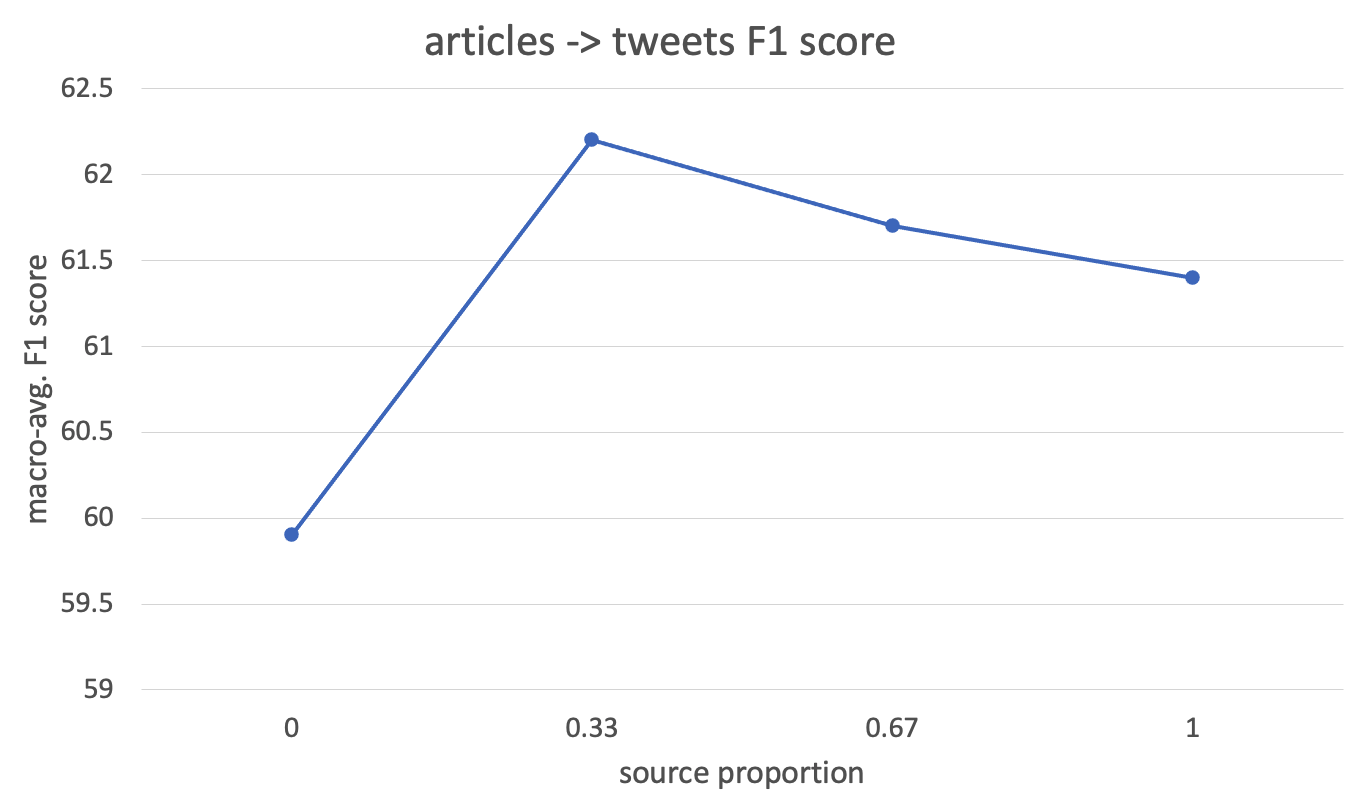
\includegraphics[scale=0.28]{0-img/nsp-ner-src-proportion-f1.png}
    \end{subfigure}
    \begin{subfigure}{\textwidth}
        \centering
        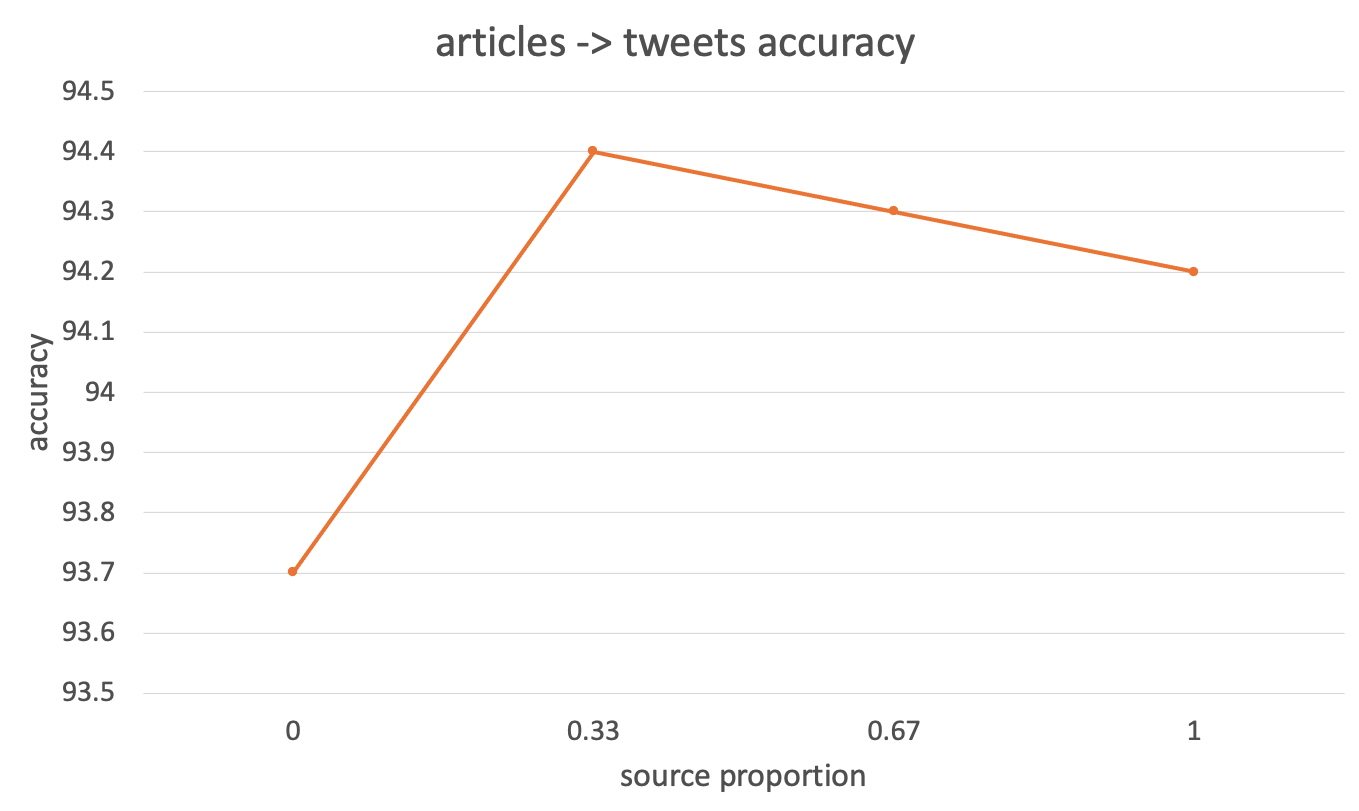
\includegraphics[scale=0.28]{0-img/nsp-ner-src-proportion-accuracy.png}
    \end{subfigure}
    \caption{Performance of extended AdaptaBERT on the NER task when varying proportion of source domain examples compared to target domain examples used in the NSP stage}
    \label{fig:nsp-ner-src-proportion}
\end{figure}

\begin{table}[ht]
    \begin{center}
        \begin{tabular}{|c|c|c|c|c|c|}
            \hline
            \multicolumn{3}{|c|}{\textbf{Task}} & \multicolumn{3}{|c|}{Bias detection} \\
            \hline
            \multicolumn{3}{|c|}{\textbf{Transfer direction}} & \multicolumn{3}{|c|}{Articles $ \rightarrow $ comments} \\
            \hline \hline
            \multicolumn{2}{|c|}{\textbf{Model Type}} & \multicolumn{2}{|c|}{\textbf{Macro-F1}} & \multicolumn{2}{|c|}{\textbf{Accuracy}} \\
            \hline
            \multicolumn{2}{|c|}{Direct transfer} & \multicolumn{2}{|c|}{54.4} & \multicolumn{2}{|c|}{51.8} \\
            \multicolumn{2}{|c|}{AdaptaBERT} & \multicolumn{2}{|c|}{58.0} & \multicolumn{2}{|c|}{59.2} \\
            \multicolumn{2}{|c|}{AdaptaBERT+NSP} & \multicolumn{2}{|c|}{58.0} & \multicolumn{2}{|c|}{58.1} \\
            \hline
            \multicolumn{2}{|c|}{In-domain} & \multicolumn{2}{|c|}{67.2} & \multicolumn{2}{|c|}{67.6} \\
            \hline
        \end{tabular}
    \end{center} \vspace{10pt}
    \begin{center}
        \begin{tabular}{|c|c|c|c|c|c|}
            \hline
            \multicolumn{3}{|c|}{\textbf{Task}} & \multicolumn{3}{|c|}{Bias detection} \\
            \hline
            \multicolumn{3}{|c|}{\textbf{Transfer direction}} & \multicolumn{3}{|c|}{Comments $ \rightarrow $ articles} \\
            \hline \hline
            \multicolumn{2}{|c|}{\textbf{Model Type}} & \multicolumn{2}{|c|}{\textbf{Macro-F1}} & \multicolumn{2}{|c|}{\textbf{Accuracy}} \\
            \hline
            \multicolumn{2}{|c|}{Direct transfer} & \multicolumn{2}{|c|}{69.6} & \multicolumn{2}{|c|}{69.3}  \\
            \multicolumn{2}{|c|}{AdaptaBERT} & \multicolumn{2}{|c|}{74.0} & \multicolumn{2}{|c|}{74.1} \\
            \multicolumn{2}{|c|}{AdaptaBERT+NSP} & \multicolumn{2}{|c|}{\textbf{73.5}} & \multicolumn{2}{|c|}{\textbf{73.5}} \\
            \hline
            \multicolumn{2}{|c|}{In-domain} & \multicolumn{2}{|c|}{76.2} & \multicolumn{2}{|c|}{76.5}  \\
            \hline
        \end{tabular}
    \end{center}
    \caption{Evaluation metrics comparing extended AdaptaBERT with optimal source:target ratio in the NSP stage to standard AdaptaBERT, direct transfer and in-domain baselines for the political bias detection task. Metrics that have improved since optimisation are highlighted in \textbf{bold}.}
    \label{tab:adaptabert-nsp-results-best}
\end{table}

\begin{table}[ht]
    \begin{center}
        \begin{tabular}{|c|c|}
            \hline
            \textbf{Task} & NER \\
            \hline
            \textbf{Transfer direction} & Articles $ \rightarrow $ tweets \\
            \hline \hline
            \textbf{Model Type} & \textbf{Macro-F1} \\
            \hline
            Direct transfer & 57.7  \\
            AdaptaBERT & 58.9  \\
            AdaptaBERT+NSP & \textbf{62.2}  \\
            \hline
            In-domain & 64.3 \\
            \hline
        \end{tabular}
    \end{center}
    \caption{Evaluation metrics comparing extended AdaptaBERT with the optimal source:target ratio in the NSP stage to standard AdaptaBERT, direct transfer and in-domain baselines for the NER task. Results 1, 2, and 4 taken from \cite{adaptabert}. Metrics that have improved since optimisation are highlighted in \textbf{bold}.}
    \label{tab:adaptabert-nsp-ner-results-best}
\end{table}

\section{Discussion}

In this chapter we have shown that extending AdaptaBERT with a Next Sentence Prediction stage yields mixed results - we achieve an improvement in classification accuracy for an NER task, but performance deterioration for the original political bias detection task.

There are a number of ways we could extend our research here. We could experiment with having more source domain than target domain material in the NSP stage - we only evaluate using no source domain material through to matching the amount of target domain material present. We could also evaluate our extended AdaptaBERT model on the POS tagging task used in the original paper \cite{adaptabert}. As mentioned in Section \ref{subsec:adaptabert-evaluation}, Han \& Eisenstein extend their MLM training corpus with an extra 1 million unlabeled tweets, which provides an extra boost in performance. Further work can be done evaluating our extended model with a larger scale cross-domain Reddit dataset. We could also experiment further with our hypothesis in Section \ref{sec:nsp-evaluation-ner} that NSP can improve performance when the source and target domain have a similar number of sentences per training example.